\documentclass[12pt]{article}
\usepackage{graphicx}
\begin{document}
    \begin{enumerate}
        \item

            \frame{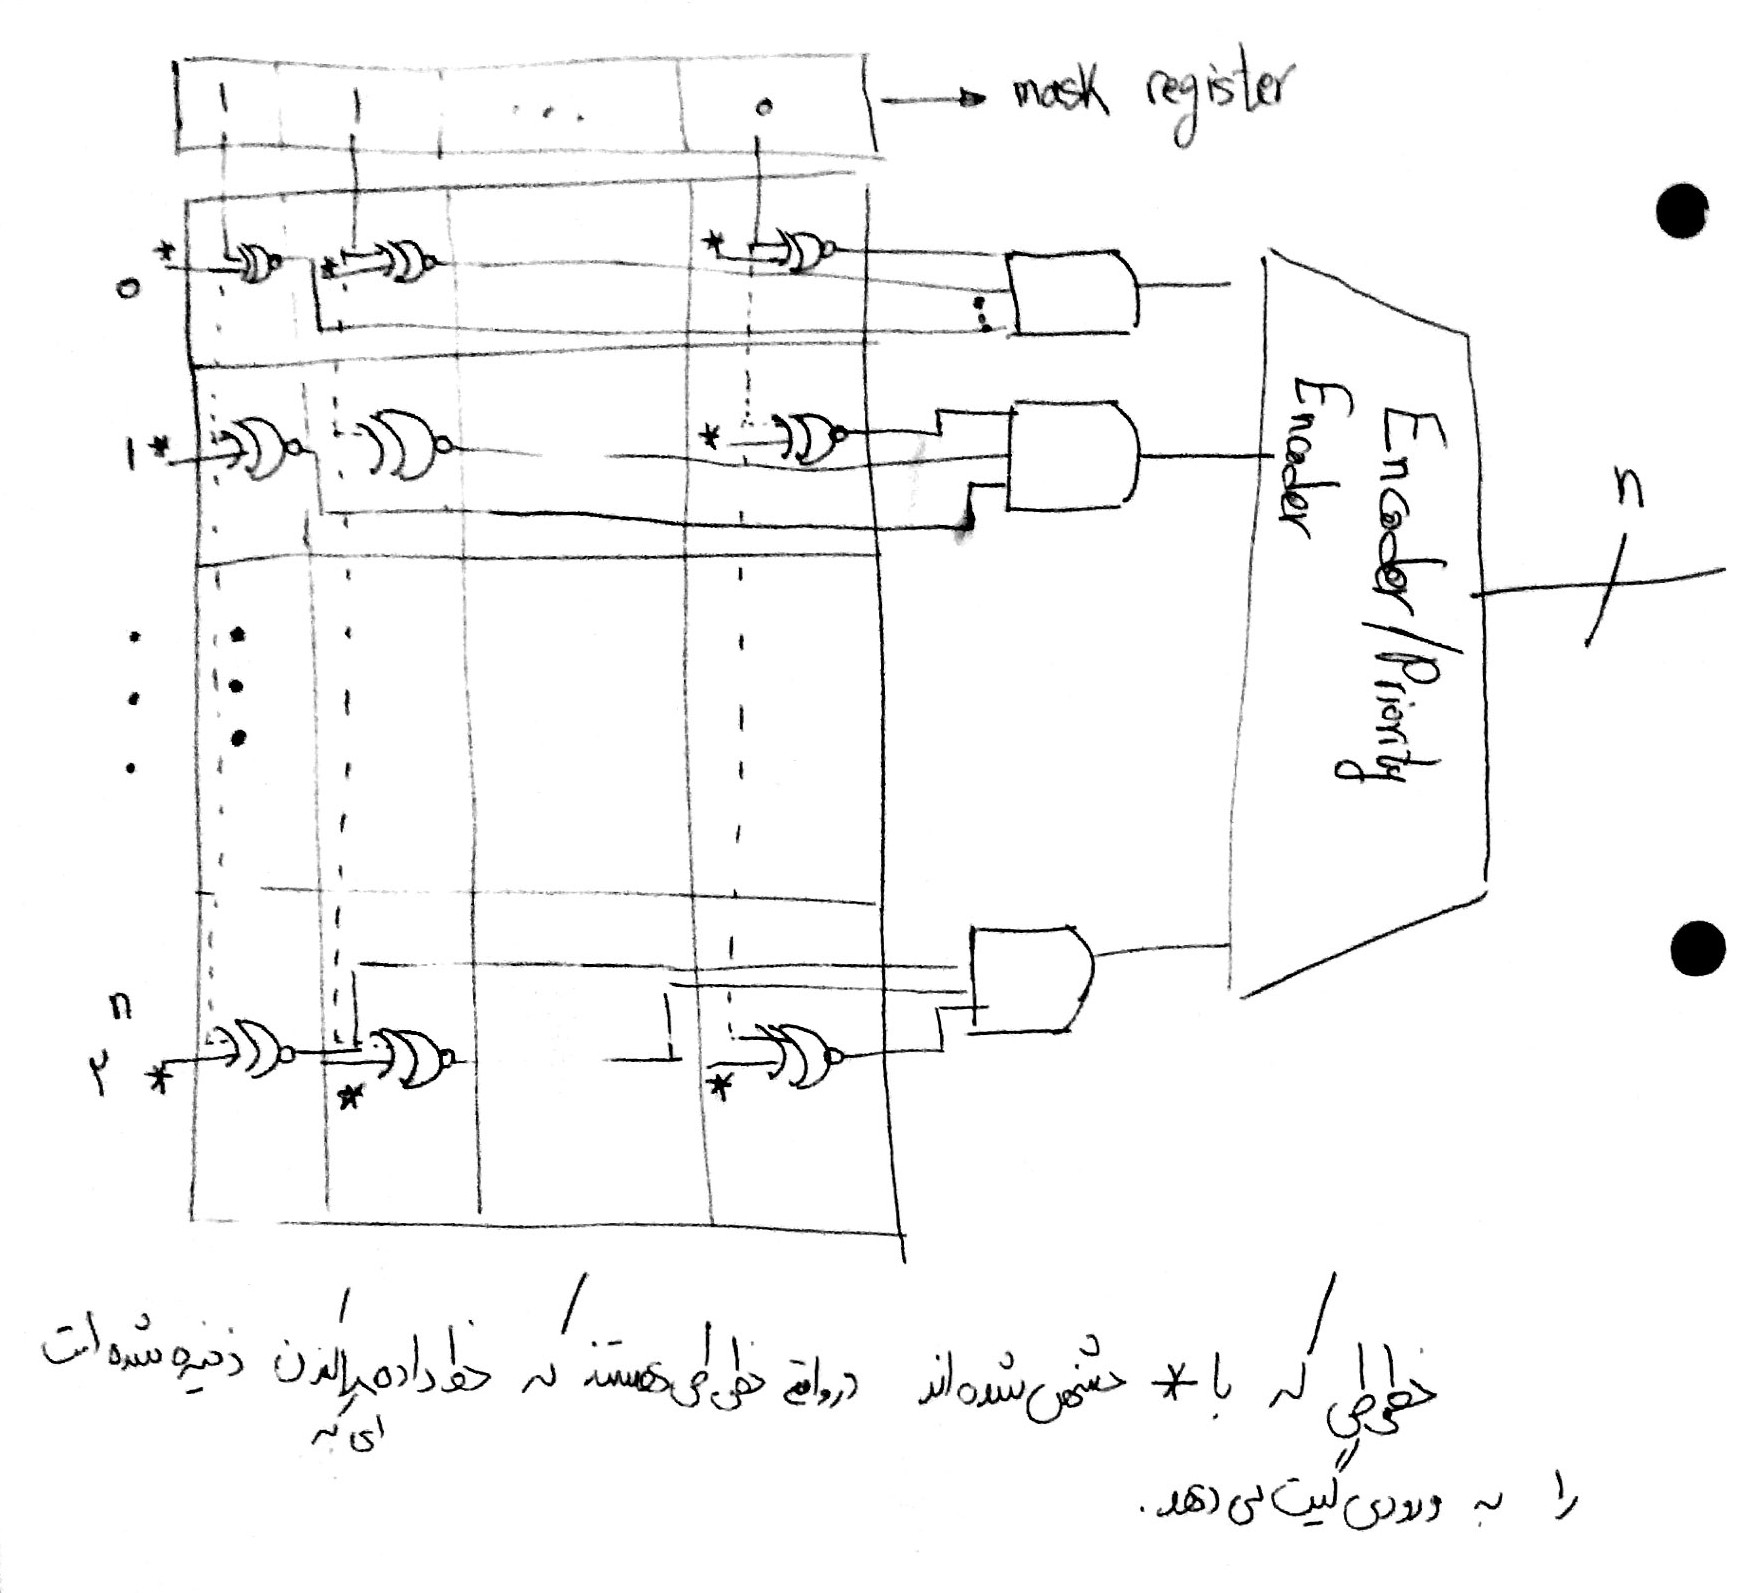
\includegraphics[scale=0.25]{CA.jpg}}
            The delay of this structue is equal to an AND gate with a fan-in equal
            to the height of the memory and a XNOR gate and the delay of the encoder.
            The cost of this structure is equalt to the number of gates used in the
            above structure.
            As shown in the logic diagram above the this memory uses XNORs to
            determine the equality of the current cell with the values of the
            mask register, And by using an AND gate it can determine whether this
            line is like the mask register or not. Then this the result line
            goes to the encoder and the result set is available.
            For using CAM with more capabilites you can use priority encoder for
            and your custom results will appear in the output.

        \item
            \begin{enumerate}
                \item
                    Because it's denser than DRAM, we can store more information
                    in it than DRAM. (And also Because it's price is the same.)
                \item
                    The problem of the low speed can be solved by using this
                    hierarchy, but the problem of limitations of writing won't
                    be solved by using this hierarchy because the memory hierarchy
                    only solves the problems caused by more speed with great cost
                    and less cost with less speed memories. But this problem will
                    not be solved by using this hierarchy.Howerver this problem
                    can be reduced by using this device as the least speed device
                    in the bottom of this hierarchy, Becasue this we reduce the
                    size of requests to this magic RAM and by this way we may
                    make the device live longer.
            \end{enumerate}
    \end{enumerate}
\end{document}
